%Dies ist die Hauptseite des Dokumentes. Es werden u. a. alle Kapitel, Einstellung im Header eingebunden.
%Ver�nderungen m�ssen in folgenden Dateien vorgenommen werden:
			%- Layout.tex 
			%- newComments.tex
			%- Titelseite
			%- Versions�bersicht
			%- einzelne Kapitel (evtl. erweitern) 
			
% Definition von globalen Parametern, die derzeit auf der Titelseite und in der Kopfzeile 
% verwendet werden. Der in <> gesetzte Text ist zu ver�ndern.  

\newcommand{\praktikumTitel}{<Titel des Praktikums>}
\newcommand{\projektTitel}{<Titel des Teilprojektes>}


%Hier sind alle Einstellungen enthalten, die sich auf das Seiten- und Dokumentenlayout beziehen

\documentclass[
	11pt,								% Schriftgr��e
	DIV12,
	german,							% f�r Umlaute, Silbentrennung etc.
	oneside,						% einseitiges Dokument
	titlepage,					% es wird eine Titelseite verwendet
	halfparskip,				% Abstand zwischen Abs�tzen (halbe Zeile)
	normalheadings,			% Gr��e der �berschriften verkleinern
	tablecaptionabove,	% Beschriftung von Tabellen unterhalb ausgeben
	final								% Status des Dokuments (final/draft)
]{scrreprt}						% 


%------�ndern von Schriftschnitten - (Muss ganz am Anfang stehen !) -------------
\usepackage{fix-cm}

%------Umlaute ------------------------------------------------------------------
% 	Umlaute/Sonderzeichen wie ���� k�nnen direkt im Quelltext verwenden werden.
%		Erlaubt automatische Trennung von Worten mit Umlauten.
\usepackage[T1]{fontenc}								 
\usepackage[latin1]{inputenc}

%------Anpassung der Landessprache-----------------------------------------------
\usepackage{ngerman}

%------Einfache Definition der Zeilenabst�nde und Seitenr�nder-------------------
\usepackage{geometry}
\usepackage{setspace}
\usepackage{tocbasic}

%------Schriftgr��enanpassung von einzelnen Textpassagen-------------------------
\usepackage{relsize}

%------Trennlinien in Kopf- und Fusszeile
\usepackage[headsepline, footsepline, ilines]{scrpage2}

%------Grafiken------------------------------------------------------------------
\usepackage{graphicx}
\usepackage{float}

%------Packet zum Sperren, Unterstreichen und Hervorheben von Texten------------
\usepackage{soul}

%------erg�nzende Schriftart----------------------------------------------------
\usepackage{helvet}

%------Lange Tabellen-----------------------------------------------------------
\usepackage{longtable}
\usepackage{array}
\usepackage{ragged2e}
\usepackage{lscape}

\usepackage{xparse}
\usepackage{framed}
\usepackage[usenames,dvipsnames]{color}

%------PDF-Optionen-------------------------------------------------------------
\usepackage[
	bookmarks,
	bookmarksopen=true,
	colorlinks=true,
	linkcolor=black,				% einfache interne Verkn�pfungen
	anchorcolor=black,			% Ankertext
	citecolor=black, 				% Verweise auf Literaturverzeichniseintr�ge im Text
	filecolor=black, 				% Verkn�pfungen, die lokale Dateien �ffnen
	menucolor=black, 				% Acrobat-Men�punkte
	urlcolor=black, 				% Farbe f�r URL-Links
	backref,								% Zur�cktext nach jedem Bibliografie-Eintrag als Liste von �berschriftsnummern
	pagebackref,						% Zur�cktext nach jedem Bibliografie-Eintrag als Liste von Seitenzahlen
	plainpages=false,				% zur korrekten Erstellung der Bookmarks
	pdfpagelabels,					% zur korrekten Erstellung der Bookmarks
	hypertexnames=false,		% zur korrekten Erstellung der Bookmarks
	% linktocpage 						% Seitenzahlen anstatt Text im Inhaltsverzeichnis verlinken
	]{hyperref}



			% enth�lt eingebundene Packete

%------Seitenr�nder-------------------------------------------------------------
\geometry{verbose, 										% zeigt die eingestellten Parameter beim Latexlauf an
			paper=a4paper, 									% Papierformat			
			top=25mm, 											% Rand oben
			left=25mm, 											% Rand links
			right=25mm, 										% Rand rechts
			bottom=45mm, 										% Rand unten
			pdftex													% schreibt das Papierformat in dei Ausgabe damit Ausgabeprogramm Papiergr��e erkennt		
	} 
	
%Seitenlayout
\onehalfspace        % 1,5-facher Abstand  

%------Kopf- und Fu�zeilen ------------------------------------------------------
\pagestyle{scrheadings}

%------Kopf- und Fu�zeile auch auf Kapitelanfangsseiten -------------------------
\renewcommand*{\chapterpagestyle}{scrheadings}

%------Schriftform der Kopfzeile ------------------------------------------------
\renewcommand{\headfont}{\normalfont}

%------Kopfzeile-----------------------------------------------------------------
\setlength{\headheight}{21mm}				% H�he der Kopfzeile
\ihead{\large{\textsc{\praktikumTitel}}\\		% Text in der linken Box
			 \small{\projektTitel}}
\chead{}														% Text in der mittleren Box

%----Fusszeile
\cfoot{}														% Text in mittlerer Box
\ofoot{\pagemark}										% Seitenzahl in rechter Box			





					% Diese Datei enth�lt alle Layouteinstellungen

%------Beginn des Gesamtdokumentes--------------------------------------------------------
\usepackage[ngerman]{babel}
\begin{document}
\shorthandoff{"}
%------Eingebundene Seiten, Verzeichnisse bzw. Kapitel------------------------------------
%----Stil dieser Seite--------------------------------------------------------------------
\thispagestyle{plain}			% Kopfzeile bleibt leer

%----Beginn der Titelseite----------------------------------------------------------------
\begin{titlepage}

%----zentrierte Ausrichtung �ber die gesamte Seite----------------------------------------		
\begin{center}

%----Titel des Praktikum (\praktikumTitel in newComments zu ver�ndern)--------------------
{\relsize{4}{\textbf{\textsc{\praktikumTitel}}}}\\[5ex]

%----Titel des Teilprojektes (\projektTitel in newComments ver�ndern)---------------------
{\relsize{3}{\textbf{\textsc{\projektTitel}}}}\\[5ex]

Praxis der Softwarentwicklung\\
Sommersemester 2014\\[6ex]

{\relsize{3}\so{\textbf{Qualit�tssicherung}}}\\[5ex]

%----Titelbild------------------------------------------------------------

\includegraphics[scale=0.25]{bilder/logo.png}\\[5ex]

%----Daten des Auftraggebers
Auftraggeber\\[2ex]															
KIT - Karlsruher Institut f�r Technologie\\
Fakult�t f�r Informatik\\										
Institut f�r Anthropromatik und Robotik (IAR)\\
Intelligente Prozessautomation und Robotik (IPR)\\[2ex]
Betreuer: Andreas Bihlmaier\\
andreas.bihlmaier@gmx.net\\[5ex]

% ----Tabelle Teilnehmer---------------------------------------------------
Auftragnehmer\\

\begin{tabular}{l<{\hspace{20mm}} l<{\hspace{30mm}}}\\	
	Name 									& 	E-Mail-Adresse\\			% Zeilen�berschift
		
	\hline										% Linie unterhalb der Zeilen�berschrift
	
	%----Nachfolgend alle Namen und E-Mail-Adressen der Teilnehmer einf�gen	
	Alex Weber & alex.weber3@gmx.net\\
	Matthias Hadlich & matthias.hadlich@student.kit.edu\\
	Matthias Klatte	& matthias.klatte@go4more.de\\
	Micha Wetzel & micha.wetzel@student.kit.edu\\	
	Sebastian Kneipp &	sebastian.kneipp@gmx.net
	
	
\end{tabular}\\[2ex]

\end{center}

\vfill Karlsruhe, 22.09.2014

\end{titlepage}
											% Titelseite	
% %kp ob wir des brauchen

%----�berschrift------------------------------------------------------------
{\relsize{2}\textbf{Versions�bersicht}}\\[2ex] 	

%----Start der Tabelle------------------------------------------------------
\begin{longtable}{|m{1.78cm}|m{1.59cm}|m{2.86cm}|m{1.9cm}|m{5.25cm}|}

	\hline																							% Linie oberhalb	
	
	%----Spalten�berschriften------------------------------------------------
	\textbf{Version}	&		\textbf{Datum}	&		\textbf{Autor}	&		\textbf{Status}	&		\textbf{Kommentar}	\\	%Spalten�berschrift	
	\hline																							% Gitterlinie
	
	%----die nachfolgeden beiden Zeilen so oft wiederholen und die ... mit den entsprechenden Daten zu f�llen wie erforderlich
	...		&		...		&		...		&		...		&		...\\				% Eintrag in Zeile
	\hline																							% Gitterlinie unten
	
%----Ende der Tabelle------------------------------------------------------	
\end{longtable}

				% Versions�bersicht
\chapter{Einleitung}

Das Robot Operating System (ROS) ist eine Middleware, um flexible Robotik
Software zu schreiben. 2007 begann Willow Garage mit der Entwicklung von ROS,
welches heute in der Robotik Community weit verbreitet ist.
Es liefert eine Sammlung von Tools, Libraries und Konventionen, welche das
Erstellen von komplexer und robuster Robotik Software auf verschiedenen
Platformen erleichtern soll.
ROS gliedert die Algorithmen zur Realisierung intelligenter Roboter in einzelne
Aufgaben, welche durch jeweils einen Prozess (Node) dargestellt und auf mehrere
Rechner (Hosts) verteilt sein k�nnen.
Die Nodes verbinden sich nach dem Publisher-Subscriber Schema �ber ein Netzwerk
miteinander, um die Datenfl�sse herzustellen (ROS Graph).

\begin{figure}[H] \centering 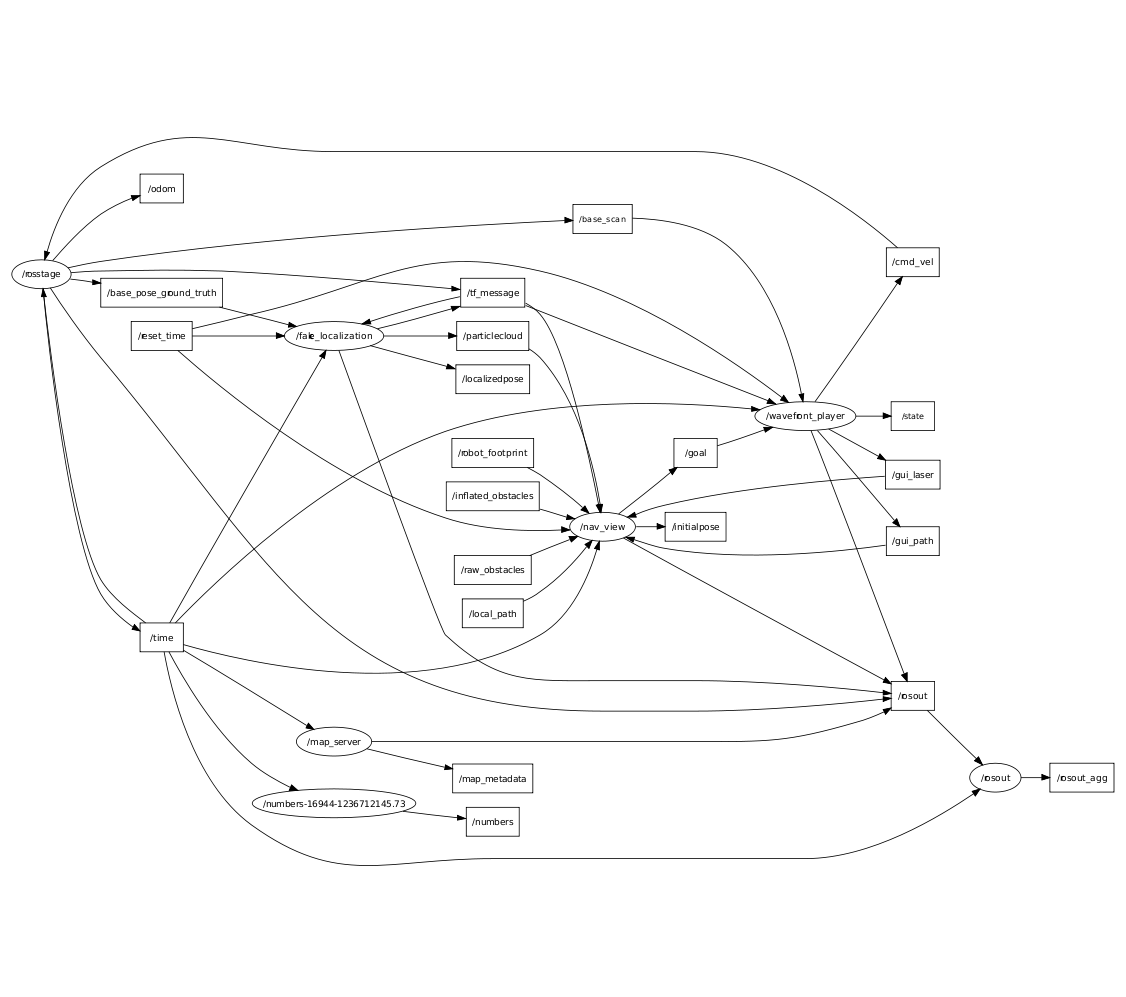
\includegraphics[scale=0.35]{./bilder/rxgraph.png}
\caption{Beispiel eines ROS Graph. Nodes sind als Ellipsen, Topics als Rechtecke
und Datenfluss als Pfeile dargestellt.
Quelle: http://www.willowgarage.com }
\end{figure}

Ein Problem stellt die �berwachung dieses Systems dar. Zwar besteht im Moment
die M�glichkeit, das Gesamtsystem auf Fehler zu �berpr�fen, jedoch ist es nicht
m�glich zu bestimmen, welcher Knoten sich fehlerhaft verh�lt. Dies kann
besonders bei gro�en System mit hunderten von Knoten zum Problem werden. Um ein
schnelles Debuggen zu erm�glichen, bedarf es einer Software zum dezentralen
Erfassen der Fehlerursachen.

Unser Ziel als PSE-Team ist es, ein System zur Definiton des Soll-Zustandes und
zum �berwachen des Ist-Zustandes individueller Knoten zu erstellen.

\tableofcontents													% Inhaltsverzeichnis wird automatisch generiert
\newpage
% \listoffigures														% ebenso das Abbildungsverzeichnis					

%----Kapitel des Feinentwurfs, die mit Inhalt zu f�llen sind------------------------------

\chapter{Zielbestimmung}

Die zu entwickelnde Softwarel�sung soll sich als �berwachungsinstrument in die Robot Operating System (ROS) Middleware einf�gen. Dabei soll �berwacht werden, ob jeder Prozess, der im ROS-Netzwerk enthalten ist, definierten Sollwerten entsprechend ordnungsgem�� Daten �bermittelt.\\
Gerade durch die gegebene Problematik eines auf mehrere Hosts verteilten Systems, bereitet das Erfassen und Verstehen von auftretenden Problemen zum aktuellen Stand des ROS Schwierigkeiten. Das vorliegende Projekt erfasst den Ist-Zustand der Prozesse im ROS-Netzwerk ohne Leistungseinbu�en kontinuierlich und visualisiert diesen im Vergleich zu definierten Soll-Werten. Auftretende Fehler und Abweichungen der von den Spezifikationen werden den Benutzer deutlich angezeigt. Es lassen sich Gegenma�nahmen f�r verschiedene Fehler definieren.\\

\section{Musskriterien}
\begin{itemize}
	\item Minimale Erweiterung bestehender Knoten zur �bermittlung von Metadaten
	\item Publizierung der Metadaten mit defnierter Frequenz auf Topics
	\item Deaktivierung der Datenerfassung einzelner Knoten
	\item Definition von Soll-Zust�nden
	\item Graphische �bersicht �ber Abweichungen von Soll- und Ist-Zustand der Knotendaten
	\item Statuserfassung der Host-Computer
\end{itemize}

\section{Wunschkriterien}
\begin{itemize}
	\item �berwachung weiterer ROS Bestandteile: Service, Parameters
	\item Selbstkontrolle der Knoten
	\item Ist-Zustand als Soll-Zustand definieren
	\item Erg�nzende �bersichten mit dem ROS Graphen und Plots �ber den zeitlichen Verlauf
\end{itemize}

\section{Abgrenzungskriterien}
\begin{itemize}
	\item Das Projekt wird keine vollst�ndige Automatisierung in Fehlerf�llen umsetzen.
	\item �berwachung der Netzwerkinfrastruktur
	\item Die Metadatenerfassung umfasst nur Knoten die daf�r modifiziert werden.
\end{itemize}
	
% \chapter{Produktfunktionen}
Produktfunktionen hier\\
\\
also was kann unser produkt kleine beschreibung
						
\chapter{Produkteinsatz}

\section{Anwendungsbereiche}
Angewandt wird die Software zum Suchen von Fehlern und �berwachen kompletter ROS Netzwerke.

\section{Zielgruppen}
Die Zielgruppe besteht aus Entwicklern und Administratoren von Umgebungen, in denen ROS eingesetzt wird. Es wird technisches Verst�ndnis der Nutzer vorausgesetzt. 

\section{Betriebsbedingungen}
\begin{itemize}
\item Zur Fehlererkennung wird die Software gestartet, um eine genauere Ursache des Fehlers festzustellen.
\item W�hrend des Produktivbetriebs wird die �berwachung zugeschaltet, um Versagen in dem System zu erkennen und automatische Gegenma�nahmen einzuleiten.
\end{itemize}

\chapter{Produktumgebung}

\section{Software}
\subsection{Implementierung}
\begin{itemize}
  \item GNU/Linux (Ubuntu 12.04) oder neuer
  \item ROS Hydro oder neuer
  \item Python 2.7.3
  \item QT 4.8
  \item PyQT 4.9.1
\end{itemize}

\subsection{Dokumentation}
\begin{itemize}
  \item Latex
  \item Pydoc
\end{itemize}

\section{Lizenz}
Das Projekt wird BSD-Lizensiert. Sollte das durch den Einsatz bestimmter Bibliotheken nicht m�glich sein, wird die n�chstm�gliche freie Open-Source Lizenz, welche sich mit der Bibliothek vereinbaren l�sst, eingesetzt.

\chapter{Funktionale Anforderungen}
das sind die von der letzten gruppe 
hab den inhalt mal drinn gelassen damit wir unser zeug einfach nur einf�gen
m�ssen


Erkl�rungen zu den OpenCV spezifischen Begriffen werden im Glossar gegeben.

\section{API \small{\textit{Pflicht}}}

\subsection{Allgemein}
\begin{description}
	\item[/FA0100/] Globale Auswahl zwischen Debug- und Release-Modus
	\item[/FA0200/] Auswahl der Visualisierung f�r jeden Operationstyp
\end{description}

\subsection{Unterst�tzung folgender Operationen von OpenCV}
\begin{description}
		\item[/FA0210/] dilate
		\item[/FA0220/] erode
		\item[/FA0230/] morphologyEx
		\item[/FA0240/] Sobel\\

		\item[/FA0250/] threshold
		\item[/FA0260/] adaptiveThreshold
		\item[/FA0270/] floodFill\\

		\item[/FA0280/] KeyPoint 
		\item[/FA0290/] DMatch
\end{description}


\section{API \small{\textit{Optional}}}

\subsection{Allgemein}
\begin{description}
	\item[/FA0300/] Optionale Parameter f�r Einstellungen der Visualisierungen
	\item[/FA0400/] Lokale Auswahl Debug/Release-Modus
	\item[/FA0500/] Optionale nicht-blockierende Aufrufe f�r Streaming
\end{description}

\subsection{Unterst�tzung folgender Operationen}

\begin{description}
	\item[/FA0600/]  stitching
	\item[/FA0610/]  ocl (OpenCL)\\

 	\item[/FA0620/] calcHist\\

	\item[/FA0630/] Canny
	\item[/FA0640/] HoughCircles
\end{description}


\section{GUI \small{\textit{Pflicht}}}
\begin{description}
	\item[/FA0700/] Eine Visualisierung pro oben gelisteter Operation (siehe API Kriterien)
	\item[/FA0800/] Drei Visualisierungen f�r features2d/DMatch (drei der m�glichen Wunsch-Visualisierungen, siehe unten)
	\item[/FA0900/]  Zoomfunktion
\end{description}

\section{GUI \small{\textit{Optional}}}

\begin{description}
	\item[/FA1000/] Permanente GUI mit Historie
	\item[/FA1200/] M�glichkeit eine Filteroperation mit ge�nderten Parametern erneut anzuwenden
	\item[/FA1300/] Hohe Zoomstufen mit Zusatzinformationen (z.B. Pixelwerte)
	\item[/FA1400/] Optionale Ausnutzung von mehreren Bildschirmen durch Fenstermodus
	\item[/FA1500/] Interaktive �berlagerung der Bilder durch Zusatzinformationen (Mouse over)
	\item[/FA1600/] Flexibler Umgang mit unterschiedlichen Bildschirm- und Bildaufl�sungen
	\item[/FA1700/] Suchleiste f�r alle Tabellen (z.B. jener der �bersichtsseite oder der Rohdatendatenanzeige)
	\item[/FA1710/] Spezielle Syntax zum Beispiel zur Gruppierung von Datens�tzen
\end{description}

\section{M�gliche Visualisierungen}

\subsection{Allgemein}
\begin{description}
	\item[/FA1800/] Darstellung von Rohdaten
	\item[/FA1810/] Abmessungen der Bilder
	\item[/FA1820/] Farbraum der Bilder (der in OpenCV genutzte Datentyp)
	\item[/FA1830/] Tabellarische Darstellung, z.B. der Matches, mit Filterm�glichkeit
	\item[/FA1840/] Diagramme (wie Histogramme)
	\item[/FA1900/] Darstellung der Bilder nebeneinander
\end{description}

\subsection{Visualisierungen von Matches}
\begin{description}
	\item[/FA2010/] Einzeichnen der Keypoints in die Bilder
	\item[/FA2020/] Verbinden der Matches durch Linien oder Pfeile
	\item[/FA2030/] Einf�rben der Linien, Pfeile oder Punkte mit Falschfarben
	\item[/FA2040/] Ausblenden der Keypoints ohne Matches
	\item[/FA2050/] Auswahl von Matches anhand bestimmter Kriterien (z.B. via Histogramm)
	\item[/FA2060/] Manuelle Auswahl von Matches
	\item[/FA2070/] Automatische Zusammenfassung von Matches zu Gruppen\\
	
	\item[/FA2110/] Einzeichnen von Linien / Formen
	\item[/FA2120/] Ausw�hlen von zugeh�rigen Matches
	\item[/FA2130/] Die Linien / Formen werden auf das zweite Bild projiziert
	\item[/FA2140/] Automatische Gruppierung der Matches zu Fl�chen\\
	
	\item[/FA2210/] Pfeill�nge und Richtung entsprechen der jeweiligenTranslation\\
	
	\item[/FA2310/] Pixelfarbwerte entsprechen den jeweiligen Tiefenwerten
\end{description}

\subsection{Visualisierungen f�r Filter}

\begin{description}
	\item[/FA2400/] Differenzbilder
	\item[/FA2500/] �berlagerungen
	\item[/FA2600/]  Direkte Anwendung von Filtern auf ein oder zwei Bilder 
		Beispiel: Anwendung eines Kantenfilters um die Auswirkungen z.B. einer Kantengl�ttung zu visualisieren
	\item[/FA2700/] Visualisierung �ber die Auswirkungen auf bestimmte Bildmetriken 
		Beispiel: �berlagerung von Histogrammen beider Bilder oder Vergleich der Kontrastwerte von bestimmten Bildbereichen
\end{description}



\newcounter{nfc}
\newcounter{nfcsec}
\newcounter{tempsec}
\setcounter{nfc}{0}
\setcounter{nfcsec}{0}

\newcommand{\nf}
{
\addtocounter{nfc}{100}
\setcounter{nfcsec}{0}

\ifnum\value{nfc}<1000
\item[/NF0\thenfc/]
\else
\item[/NF\thenfc/]
\fi
}

\newcommand{\nfsec}
{
\addtocounter{nfcsec}{10}
\setcounter{tempsec}{\thenfc}
\addtocounter{tempsec}{\thenfcsec}
\ifnum\value{nfc}<1000
\item[/NF0\thetempsec/]
\else
\item[/NF\thetempsec/]
\fi
}





\chapter{Nichtfunktionale Anforderungen}
\section{Produktleistungen \small{\textit{Pflicht}}}
\begin{description}
\nf
\nfsec
\nf
	\item[/NF0100/] Die GUI soll schnell starten und interaktiv bedienbar sein
	\item[/NF0200/] M�glichst kein Overhead im Release-Modus
\end{description}

\section{Produktleistungen \small{\textit{Optional}}}
\begin{description}
	\item[/NF0300/] Flexibler Umgang mit unterschiedlichen Bildschirm- und Bildaufl�sungen
	\item[/NF0400/] Integration in das OpenCV Test Framework
\end{description}

\section{Qualit�tsanforderungen \small{\textit{Pflicht}}}
\begin{description}
	\item[/NF0500/] Keine signifikanten Speicherlecks
	\item[/NF0600/] Erweiterbarkeit um zus�tzliche OpenCV Operationen und Visualisierungen
	\item[/NF0700/] Modularer Aufbau (API und GUI)
	\item[/NF0900/] Einhaltung der OpenCV und Qt Konventionen
	\item[/NF1000/] Ausf�hrliche Dokumentation der API und des GUI
\end{description}

\section{Qualit�tsanforderungen \small{\textit{Optional}}}
\begin{description}
	\item[/NF1100/] Dokumentation des internen Codes mit Werkzeug
	\item[/NF1200/] OpenCV geeigneter Aufbau des Build-Systems
	\item[/NF1300/] Abdeckung durch Tests
	\item[/NF1400/] Keine Resource-Leaks
	\item[/NF1500/] Threadsafety \small{\textit{Im C++11-Modus}}
	\item[/NF1600/] Toleranz gegen�ber fehlerhaften API-Aufrufen
	\item[/NF1700/] Kein undefiniertes Verhalten
\end{description}

\chapter{Produktdaten}

hier bin ich mir nicht ganz so sicher was genau rein muss
\chapter{Systemmodell}

\section{Szenarien}

\subsection*{Darstellung von Fehlern}
\subsubsection*{Fehlerfeststellung durch den Benutzer}
\begin{itemize}
	\item Einem Benutzer ist ein Fehler aufgefallen: Der Roboter verh�lt sich nicht mehr, wie erwartet wird.
	\item Er �ffnet das PSE Introspection Plugin in der rqt GUI.
	\item Sofort sieht er, dass das Plugin den Fehler erfasst hat. Es zeigt ein Problem an.
	\item In einer Knoten�bersicht f�llt es dem Benutzer leicht, die farblich auff�llig hinterlegten fehlerhaften Knoten auszumachen.
	\item Er �ffnet die betroffenen Knoten in der Detailansicht und sieht, in welchen Punkten das Knotenverhalten von den Spezifikationen abweicht.
\end{itemize}
\subsubsection*{Fehlerfeststellung �ber die GUI}
\begin{itemize}
	\item Um den Status des ROS-Netzwerkes im Auge zu behalten, hat der benutzer das PSE Introspection Plugin in der rqt GUI ge�ffnet.
	\item Er stellt fest, dass die Statusanzeige nicht mehr in Gr�n volle Funktionalit�t signalisiert.
	\item Mit einem Klick �ffnet er das Fehlerlog, in dem er Eintr�ge findet, welche Knoten von ihren Spezifikationen abweichend arbeiten und die Fehlermeldung ausgel�st haben.
	\item Nun hat der Anwender die M�glichkeit, die Fehlerhaften Knoten aus einer Liste zu suchen und sie in einer Detailansicht zu �ffnen, um sich weitere Details �ber die ausgefallenen Komponenten anzeigen zu lassen.
\end{itemize}

\subsection*{Knotendetail-Ansicht}
\subsubsection*{Auswahl eines Knotens}
\begin{itemize}
	\item Der Benutzer m�chte sich die Metadaten Informationen zu einen Knoten anzeigen.
	\item Er w�hlt sich den Knoten, der ihn interessiert aus einer Liste.
	\item Dazu besteht die M�glichkeit, diesen in einer Liste zu finden, welche sich auch �ber ein Suchfeld filtern l�sst.
	\item W�hlt er einen Knoten aus, �ffnet sich ein kleines Fenster mit den Knoteninformationen und reiht sich in die �bersicht der ge�ffneten Detailfenster ein.
\end{itemize}
\subsubsection*{Umschalten der Detailansicht am Beispiel der Topic Liste}
\begin{itemize}
	\item Das Detailfenster bietet f�r verschiedene Knotendaten Links, um die Ansicht zu erweitern.
	\item Der Benutzer bekommtein Topic angezeigt, mit dem der Knoten in einem Publisher/Subscriber-Verh�ltnis steht.
	\item Klickt der Benutzer auf eine Schaltfl�che neben der Anzeige, wir die Anzeige der sonstigen Metadaten durch eine vollst�ndige Auflistung der relevanten Topics ersetzt.
	\item Intuitiv positioniert findet der Anwender eine Schaltfl�che, um zur vorigen Ansicht zur�ckzukehren.
\end{itemize}

\subsection*{Dynamische GUI}
\begin{itemize}
	\item Der Benutzer schlie�t ein rqt Plugin, das er nicht mehr ben�tigt.
	\item Daraufhin verschiebt sich das Layout in der rqt GUI und das PSE Introspection Plugin �ndert seine Form und Gr��e.
	\item Das PSE Introspection Plugin rearrangiert seine Inhalte, um sie im neuen Layout anzuzeigen.
\end{itemize}

\section{Anwenungsf�lle}

\chapter{Benutzeroberfl�che}

hier kommen dann ein paar bilder und dazugeh�rige beschreibungenen unserer gui

\begin{itemize}
	\item blasdgfs
	\item sdfg
	\item was man halt alles so allgemeines reinschreiben kann
\end{itemize}

\newpage

\begin{figure}

\section{Skizzen bzw. Bilder}

\subsection{name des bildes}
	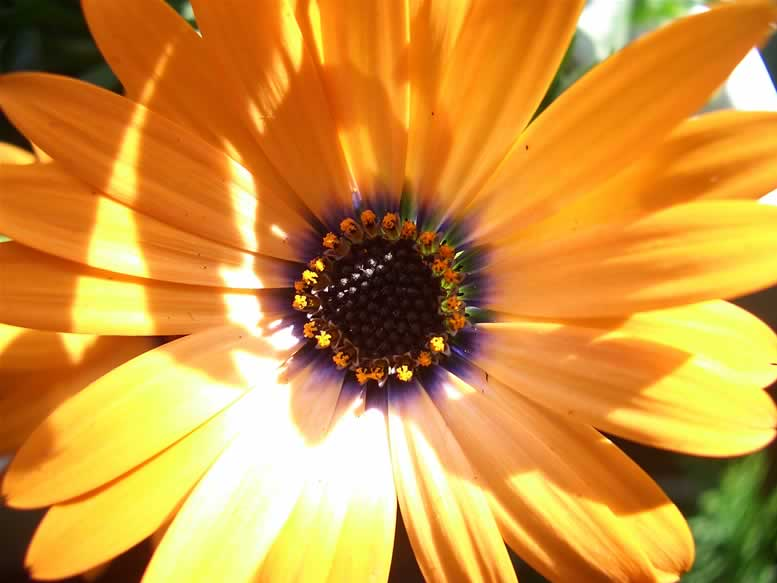
\includegraphics[width=\linewidth]{bilder/blume-beispielbild.jpg}
	\caption{bildunterschrift}
	
	Ein ganz ganz langer text zum bild\\
	kdfnakgflkadshfkjsfkljsadfjk�adshf�lkdf\\
	hsgkj�ldhflkghsfdlkgh�dklfhglkdsjgl�dshgkdsfh�gh\\
	sdflkendgkjhdsfk�ghadfsopfghaoifhaigtfuiaerhgiuag
\newpage

\end{figure}

\begin{figure}
\subsection{name des bildes}
	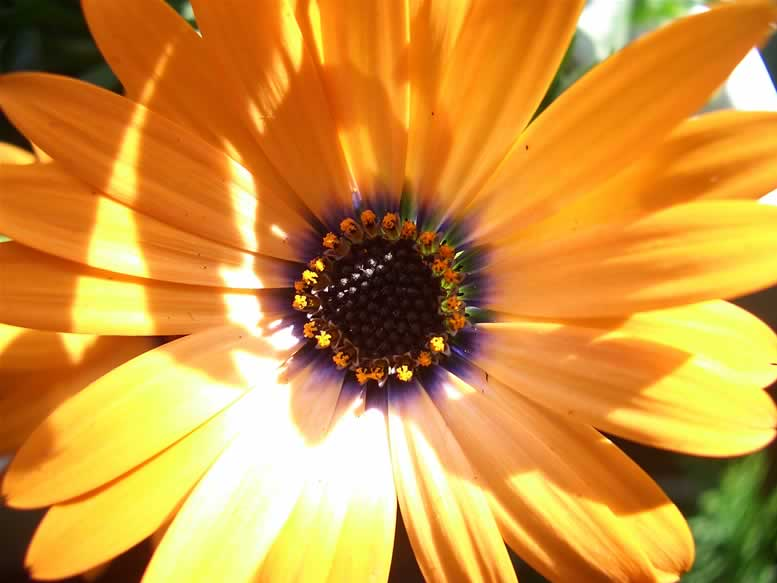
\includegraphics[width=\linewidth]{bilder/blume-beispielbild.jpg}
	\caption{bildunterschrift}
	
	Ein ganz ganz langer text zum bild\\
	kdfnakgflkadshfkjsfkljsadfjk�adshf�lkdf\\
	hsgkj�ldhflkghsfdlkgh�dklfhglkdsjgl�dshgkdsfh�gh\\
	sdflkgkjhdsfk�ghadfsopfghaoifhaigtfuiaerhgiuag
\newpage

\end{figure}
	

% Kapitel 7
%-------------------------------------------------------------------------------


\chapter{Qualit�tsanforderungen}
\newcounter{tfc}
\setcounter{tfc}{0}
\newcommand{\tf}{
	\addtocounter{tfc}{10}
	\ifnum\value{fac}<100
		\item[/TF0\thefac/]
	\else
		\item[/TF\thefac/]
	\fi
}

\chapter{Testf�lle}
\begin{description}
	\tf Es wird festgestellt, dass ein Knoten keine Daten mehr sendet
	\tf Es wird festgestellt, wenn ein Knoten langsamer oder schneller als sonst Daten sendet.\\
		Es wird festgestellt, wenn ein Knoten ma�geblich von den Sollwerten abweicht.
	\tf Eingelesene Konfigurationsdaten lassen sich parsen und auslesen
	\tf Hostdaten werden �bermittelt
	\tf rqt Plugin reagiert auf Gr��en�nderung
\end{description}
% \chapter{Entwicklungsumgebung}

\section{Implementierung}

\begin{itemize}
  \item GNU/Linux (Ubuntu 12.04)
  \item ROS Hydro oder neuer
  \item Python 2.7 oder neuer
  \item QT 5.0 oder neuer
\end{itemize}

\section{Dokumentation}

\begin{itemize}
  \item Latex
  \item Pydoc
\end{itemize}
\chapter{Glossar}
\label{sec:glossar}
\section{Allgemein}
\begin{description}
 \glossaryItem{API}{Application Programming Interface. Eine Schnittstelle, �ber die Programme auf Funktionalit�t anderer Programme zugreifen k�nnen}
 \glossaryItem{CPU}{Central Processing Unit. Das englische Akronym f�r den Prozessor eine Computers.}
 \glossaryItem{GUI}{Graphische Benuteroberfl�che, original aus dem Englischen: Graphical User Interface}
 \glossaryItem{Middleware}{Schicht, die zwischen Anwendungen und der Infrastruktur vermittelt um so die Komplexit�t der anderen Schichten zu verbergen}
 \glossaryItem{Open Source}{Software die Quelloffen ist und weiterentwickelt sowie weiterverbreitet werden darf} 
 
\end{description}
\section{ROS}
\begin{description}
 \glossaryItem{Knoten}{Siehe Node}
 \glossaryItem{Master}{Der Master erm�glicht die Namensaufl�sung und -registrierung und ist zust�ndig f�r die Verkn�pfung von Knoten miteinander.}
 \glossaryItem{Message}{Nachricht, welche zwischen Knoten versendet wird. Eine Nachricht besteht aus primitiven Datentypen.} 
 \glossaryItem{Node}{Auch Knoten genannt. Repr�sentiert ein Prozess. Erm�glicht verschiedene Aufgaben zu trennen und so das ROS Netzwerk modular zu gestalten.}
 \glossaryItem{Parameter Server}{Der Parameter Server erlaubt das zentrale Speichern von Daten. Alle Knoten k�nnen auf ihn zugreifen.}
 \glossaryItem{Publisher}{Objekt, das Messages unter bestimmten Topics ver�ffentlicht}
 \glossaryItem{ROS}{Das Robot Operating System ist eine Open-Source Middleware um flexible Robotik Software zu schreiben}
 \glossaryItem{Service}{Services dienen zur zweiwege Kommunikation in ROS Netzwerken, da das Publisher/Subscriber System nur einwege Kommunikation unterst�tzt. Services verhalten sich wie entfernte Funktionsaufrufe (RPC).}
 \glossaryItem{Subscriber}{Objekt, das Messages von abonnierten Topics empf�ngt }
 \glossaryItem{Topic}{Ein Topic ist ein Name um den Inhalt einer Message zu definieren. Publisher k�nnen Messages auf bestimmten Topics publizieren, Subscriber k�nnen Messages von abonnierten Topics erhalten}
\end{description}

% \chapter{Literatur}
same here das von letztem jahr

\begin{description}
	\item[Designed for Use -- Create Usable Interfaces for Applications and the Web / Lukas Mathis]
	Die vorliegenden GUI-Entw�rfe sind stark von diesem Buch beeinflusst, da es wichtige Techniken, Methoden und Denkmuster der UI-Entwicklung vermittelt. \textit{Und das in einer f�r Informatiker verst�ndlichen Sprache.}
	\item[\href{http://docs.openCV.org}{OpenCV Dokumentation}]
	Eine wichtige Quelle aus offensichtlichen Gr�nden.
	\item[Technisches Schreiben -- (nicht nur) f�r Informatiker / Peter Rechenberg]
	Ein anschaulich und verst�ndlich geschriebenes Buch, das hilft den eigenen Schreibstil zu verbessern. Und damit die Verst�ndlichkeit der geschriebenen Dokumentation (vgl. \nameref{produktdaten}) zu erh�hen.
\end{description}		
				

%------Ende des Dokumentes----------------------------------------------------------------
\end{document}
